\documentclass[11pt, oneside]{article}

\pdfoutput=1

\RequirePackage[utf8]{inputenc}
\RequirePackage[T1]{fontenc}
\RequirePackage{xcolor,graphicx}
\RequirePackage{hyperref}
\hypersetup{%
  colorlinks=true,
  breaklinks=true,
  linkcolor=red,
  anchorcolor=black,
  citecolor=brown,
  filecolor=blue,
  menucolor=red,
  urlcolor=red,
}
\RequirePackage[authoryear]{natbib}
\RequirePackage{xr}
\RequirePackage{mathtools, amsfonts, amssymb,amsthm}
\mathtoolsset{showonlyrefs}
\RequirePackage{enumerate}
\RequirePackage{comment}
\RequirePackage{ifthen}
\RequirePackage{enumerate}
\RequirePackage{comment}
\RequirePackage{subcaption}
\RequirePackage{siunitx}
\RequirePackage[ruled,vlined]{algorithm2e}

\externaldocument{ms}


\setlength{\textwidth}{16cm}
\setlength{\textheight}{22cm}
\setlength{\hoffset}{-1.4cm}
\topmargin -1cm 



%%%%%%%%%%%%%%%%%%%%%%%%%%%%%%%%%%%%%%%%%%%%%%%%%%%%%%%%%
%%%%%%%%%%% JDT:  Annotation Code %%%%%%%%%%%%%%%%%%%%%%%%%%%%%%%%%%
%%%%%%%%%%%%%%%%%%%%%%%%%%%%%%%%%%%%%%%%%%%%%%%%%%%%%%%%%

\RequirePackage{color}
\RequirePackage[normalem]{ulem}

 % Uncomment to display with annotation; comment out otherwise
\newcommand{\add}[1]{\textcolor{blue}{#1}}
\newcommand{\delete}[1]{\textcolor{red}{\sout{#1}}}
\newcommand{\edit}[2]{\textcolor{red}{\sout{#1}} \textcolor{blue}{#2}}
\newcommand{\mnote}[1]{\marginpar{\textcolor{green}{\textbf{#1}}}}


% -------------
% Some commands
% -------------

% Environment
\newcounter{rem}
\newtheorem{remark}[rem]{Remark}

\newcounter{th}
\newtheorem{theorem}[th]{Theorem}

\newcounter{lm}
\newtheorem{lemma}[lm]{Lemma}

\newcounter{scenario}[section]
\newenvironment{scenario}[1][]{\refstepcounter{scenario}\par\medskip
   \noindent \textbf{Scenario~\thescenario. #1} \rmfamily}{\medskip}

\newenvironment{results}[1][]{\noindent \textbf{#1} \rmfamily}{\medskip}

\providecommand{\keywords}[1]{\textbf{\textit{Keywords---}} #1}

% Stats
\newcommand{\EE}{\mathbb{E}} % Expectation
\newcommand{\RR}{\mathbb{R}} % R
\newcommand{\NN}{\mathbb{N}} % N
\newcommand{\XX}{\mathcal{X}} % set X
\newcommand{\dd}{{\rm d}}

% Spaces
\newcommand{\TT}[1]{\mathcal{T}_{#1}} % Domain definition space
\newcommand{\sLp}[1]{\mathcal{L}^{2}\left(#1\right)} % L^p space
\newcommand{\HH}{\mathcal{H}} % Product of L^p space
\newcommand{\GG}{\mathcal{G}} % (L^p)^N space

% Inner product and norm
\newcommand{\pointt}{\mathbf{t}} % Indexed of multivariate curves
\newcommand{\points}{\mathbf{s}} % Indexed of multivariate curves
\newcommand{\inLp}[2]{\left\langle#1, #2\right\rangle} % Inner product in Lp
\newcommand{\inR}[2]{\left(#1, #2\right)}
\newcommand{\inRM}[2]{\left(#1, #2\right)_{\mathbf{M}}}
\newcommand{\normLp}[1]{\left|\!\left|#1\right|\!\right|} % Norm in Lp
\newcommand{\normR}[1]{\left(\!\left(#1\right)\!\right)} %
\newcommand{\normRM}[1]{\left(\!\left(#1\right)\!\right)_{\mathbf{M}}} %
\newcommand{\inH}[2]{\langle\!\langle#1, #2\rangle\!\rangle}
\newcommand{\inHw}[2]{\langle\!\langle#1, #2\rangle\!\rangle_w}
\newcommand{\inHG}[2]{\langle\!\langle#1, #2\rangle\!\rangle_\Gamma}
\newcommand{\normH}[1]{\left|\!\left|\!\left|#1\right|\!\right|\!\right|}
\newcommand{\normHG}[1]{\left|\!\left|\!\left|#1\right|\!\right|\!\right|_\Gamma}

% Data/Process related
\newcommand{\Xnp}{X_n^{(p)}} % Observation n, feature p
\newcommand{\Xnq}{X_n^{(q)}} % Observation n, feature q
\newcommand{\hatXnp}{\widehat{X}_n^{(p)}} % Reconstruction
\newcommand{\Xp}[1]{X^{(#1)}} % Feature p
\newcommand{\hatXp}[1]{\widehat{X}^{(#1)}} % Reconstruction, Feature p
\newcommand{\mup}[1]{\mu^{(#1)}} % Feature p
\newcommand{\hatmup}[1]{\widehat{\mu}^{(#1)}} % Reconstruction, Feature p
\newcommand{\fp}{f^{(p)}} 
\newcommand{\gp}{g^{(p)}}

% Geometric related
\newcommand{\pobs}[1]{\mathrm{#1}} % Point related to observations
\newcommand{\CN}{\mathcal{C}_{\!N}} % Cloud of features
\newcommand{\Gmu}{\pobs{G}_{\!\mu}} % Centre of gravity of C_N
\newcommand{\OH}{\pobs{O}_{\!\mathcal{H}}} % Centre of H

\newcommand{\pfea}[1]{\mathsf{#1}} % Point related to features
\newcommand{\CP}{\mathcal{C}_{\!P}} % Cloud of observations
\newcommand{\Gfea}{\pfea{G}_{\!\mu}} % Centre of gravity of C_P
\newcommand{\OG}{\pfea{O}_{\!\RR}} % Centre of H

% Declaration of math operator
\DeclareMathOperator{\Var}{Var}
\DeclareMathOperator{\Cov}{Cov}
\DeclareMathOperator*{\argmax}{arg\,max}
\DeclareMathOperator{\bigO}{\mathcal{O}}

% Function subset restriction  
\newcommand\restr[2]{{ %
  \left.\kern-\nulldelimiterspace  %
  #1  %
  \vphantom{\big|}  %
  \right|_{#2}  %
}}
% -------------

\title{Supplementary material for ``On the use of the Gram matrix for multivariate functional principal components analysis''}

\author{%
Steven Golovkine\thanks{MACSI, Department of Mathematics and Statistics, University of Limerick, Ireland \href{mailto:steven.golovkine@ul.ie}{steven.golovkine@ul.ie}}
\and
Edward Gunning\thanks{Department of Biostatistics and Epidemiology, University of Pennsylvania, USA \href{mailto:edward.gunning@pennmedicine.upenn.edu}{edward.gunning@pennmedicine.upenn.edu}}
\and
Andrew J. Simpkin\thanks{School of Mathematical and Statistical Sciences, University of Galway, Ireland \href{mailto:andrew.simpkin@nuigalway.ie}{andrew.simpkin@nuigalway.ie}}
\and
Norma Bargary\thanks{MACSI, Department of Mathematics and Statistics, University of Limerick, Ireland \href{mailto:norma.bargary@ul.ie}{norma.bargary@ul.ie}}
}
\date{\today}

\begin{document}

\maketitle

In this Supplementary Material, we provide insights for when the data are already decomposed in a basis, e.g. Fourier or polynomials. In particular, we explain how to perform MFPCA as described in Section~\ref{sec:functional_principal_components_analysis} in the main text.

\renewcommand{\theequation}{SM.\arabic{equation}}


\section{Basis decomposition} % (fold)
\label{sub:basis_decomposition}


In many practical situations, functional data are noisy and only observed at specific time points. To extract the underlying functional features of the data, smoothing and interpolation techniques are commonly employed. These techniques involve approximating the true underlying function generating the data by a finite-dimensional set of basis functions. Assume that for each feature $p = 1, \dots, P$, there exists a set of basis of functions $\Psi^{(p)} = \{\psi_k^{(p)}\}_{1 \leq k \leq K_p}$ such that each feature of each curve $n = 1, \dots, N$ can be expanded using the basis:
\begin{equation}\label{eq:curve_basis_expansion}
\Xnp(t_p) = \sum_{k = 1}^{K_p} c^{(p)}_{nk}\psi_k^{(p)}(t_p), \quad t_p \in \TT{p},
\end{equation}
where $\{c^{(p)}_{nk}\}_{1 \leq k \leq K_p}$ is a set of coefficients for feature $p$ of observation $n$. We denote by $\overline{c}_k^{(p)} = \sum_{n = 1}^N \pi_n c^{(p)}_{nk}$ the mean coefficient of feature $p$ corresponding to the $k$th basis function.
The $p$th feature of the mean function can be then expanded in the same basis as:
\begin{equation}
    \hatmup{p}(t_p) = \sum_{k = 1}^{K_p} \overline{c}_k^{(p)}\psi_k^{(p)}(t_p), \quad t_p \in \TT{p}.
\end{equation}
Similarly, the covariance function of the $p$th and $q$th features is given by:
\begin{equation}
    \widehat{C}_{p,q}(s_p, t_q) = \sum_{k = 1}^{K_p} \sum_{l = 1}^{K_q} \left(\sum_{n = 1}^N \pi_n c^{(p)}_{nk}c^{(q)}_{nl} - \overline{c}_k^{(p)}\overline{c}_l^{(q)}\right)\psi_k^{(p)}(s_p)\psi_l^{(q)}(t_q), \quad s_p \in \TT{p},\quad t_q \in \TT{q}.
\end{equation}
These formulas can be written in matrix form as follows. For $\pointt \in \TT{}$, we have that $X(\pointt) = \mathbf{C}\Psi(\pointt)$ where $X(\pointt)$ is a $N \times P$ matrix with entries $\Xnp(t_p),~t_p \in \TT{p},~1 \leq p \leq P,~1 \leq n \leq N$,
\begin{equation}
    \mathbf{C} = \begin{pmatrix}
            \mathbf{C}^{(1)} & \cdots & \mathbf{C}^{(P)} \\
        \end{pmatrix}, \quad \text{and}\quad
    \Psi(\pointt) = \text{diag}\{\Psi^{(1)}(t_1), \dots, \Psi^{(P)}(t_P)\},
\end{equation}
where
\begin{equation}
\mathbf{C}^{(p)} = \begin{pmatrix}
    c^{(p)}_{11} & \cdots & c^{(p)}_{1K_p} \\
    \vdots & \ddots & \vdots \\
    c^{(p)}_{N1} & \cdots & c^{(p)}_{NK_p}
\end{pmatrix} \\
\quad \text{and}\quad
\Psi^{(p)}(t_p) = \begin{pmatrix}
    \psi_1^{(p)}(t_p) \\
    \vdots \\
    \psi_{K_p}^{(p)}(t_p)
\end{pmatrix}.
\end{equation}
Using the basis expansion and denoting $\Pi^\top = (\pi_1, \dots, \pi_N)$, the mean and covariance functions are given by
\begin{equation}
    \widehat{\mu}(\pointt) = \Psi(\pointt)^\top \mathbf{C}^\top\Pi \quad\text{and}\quad \widehat{C}(\points, \pointt) = \Psi(\points)^\top \mathbf{C}^\top \left(\text{diag}\{
        \pi_1, \dots, \pi_N\} - \Pi\Pi^\top\right)\mathbf{C} \Psi(\pointt).
\end{equation}
Finally, we denote by $\mathbf{W}$ the matrix of inner products of the functions in the basis $\Psi$. The matrix $\mathbf{W}$ is a block-diagonal matrix such that $\mathbf{W} = \text{blockdiag}\{\mathbf{W}^{(1)}, \dots, \mathbf{W}^{(P)}\}$ where each entry is given by
\begin{equation}
    \mathbf{W}_{k, l}^{(p)} = \inLp{\psi_k^{(p)}}{\psi_l^{(p)}}, \quad 1 \leq k, l \leq K_p, \quad 1 \leq p \leq P.
\end{equation}
We remark that, if the basis $\Psi$ is an orthonormal basis, the matrix $\mathbf{W}$ is equal to the identity matrix of size $\sum_{p = 1}^P K_p$.
Using the expansion of the data into the basis of functions $\Psi$, the inner-product matrix $\mathbf{M}$ is written 
\begin{equation}\label{eq:gram_matrix_basis}
    \mathbf{M} = \text{diag}\{
        \sqrt{\pi_1}, \dots, \sqrt{\pi_N}\}\left(\mathrm{I}_{\!N} - \mathbf{1}_{\!N}\Pi^\top\right) \mathbf{C} \mathbf{W} \mathbf{C}^\top \left(\mathrm{I}_{\!N} - \Pi\mathbf{1}_{\!N}^\top\right)\text{diag}\{
        \sqrt{\pi_1}, \dots, \sqrt{\pi_N}\}
\end{equation}
where $\mathrm{I}_{\!N}$ is the identity matrix of size $N$ and $\mathbf{1}_{\!N}$ is a vector of $1$ of length $N$.


% subsection basis_decomposition (end)


\section{MFPCA with a basis expansion} % (fold)
\label{sub:with_a_basis_expansion}

In this section, we assume that the observations are expanded into a basis of functions, as explained in Section~\ref{sub:basis_decomposition}. Using the expansion of the data into the basis of function $\Psi$ and $\mathbf{W}$, the matrix of inner products of the functions in the basis $\Psi$, we write \eqref{eq:gram_matrix_basis} as
\begin{equation}
    \mathbf{M} = \left(\text{diag}\{
        \sqrt{\pi_1}, \dots, \sqrt{\pi_N}\}\left(\mathrm{I}_{\!N} - \mathbf{1}_{\!N}\Pi^\top\right) \mathbf{C}\mathbf{W}^{1/2}\right)\left(\text{diag}\{
        \sqrt{\pi_1}, \dots, \sqrt{\pi_N}\}\left(\mathrm{I}_{\!N} - \mathbf{1}_{\!N}\Pi^\top\right) \mathbf{C}\mathbf{W}^{1/2}\right)^\top.
\end{equation}
We note
\begin{equation}
    \mathbf{A} = \text{diag}\{\sqrt{\pi_1}, \dots, \sqrt{\pi_N}\}\left(\mathrm{I}_{\!N} - \mathbf{1}_{\!N}\Pi^\top\right) \mathbf{C}\mathbf{W}^{1/2},
\end{equation}
such that $\mathbf{M} = \mathbf{A}\mathbf{A}^\top$.
We also assume that $\phi_1, \phi_2, \dots$ the eigenfunctions of the covariance operator $\Gamma$ have a decomposition into the basis $\Psi$
\begin{equation}
    \phi_k(\cdot) = 
        \begin{pmatrix} 
            \phi_k^{(1)}(\cdot) \\
            \vdots \\
            \phi_k^{(P)}(\cdot)
        \end{pmatrix} = 
        \begin{pmatrix} 
            \psi^{(1) \top}(\cdot) b_{1k} \\
            \vdots \\
            \psi^{(P) \top}(\cdot) b_{Pk}
        \end{pmatrix}, \quad\text{where}\quad
        b_{pk} = \left(b_{p k 1}, \dots, b_{p k K_p} \right)^\top.
\end{equation}
We have, for $p = 1, \dots, P$,
\begin{align*}
    \left(\Gamma \phi_k\right)^{(p)}(\cdot) &= \sum_{q = 1}^P \int_{\TT{q}} C_{p, q}(\cdot, s_q)\phi_k^{(q)}(s_q) \dd s_q \\
    &= \sum_{q = 1}^P \int_{\TT{q}} \Psi(\cdot)^{(p) \top} \mathbf{C}^{(p) \top} \left(\text{diag}\{\pi_1, \dots, \pi_N\} - \Pi\Pi^\top\right)\mathbf{C}^{(q)} \Psi^{(q)}(s_q) \Psi^{(q)}(s_q)^\top b_{q k} \dd s_q \\
    &= \Psi(\cdot)^{(p) \top} \mathbf{C}^{(p) \top} \left(\text{diag}\{\pi_1, \dots, \pi_N\} - \Pi\Pi^\top\right)\sum_{q = 1}^P \mathbf{C}^{(q)} \int_{\TT{q}} \Psi^{(q)}(s_q) \Psi(s_q)^{(q) \top} \dd s_q b_{q k} \\
    &= \Psi(\cdot)^{(p) \top} \mathbf{C}^{(p) \top} \left(\text{diag}\{\pi_1, \dots, \pi_N\} - \Pi\Pi^\top\right) \sum_{q = 1}^P \mathbf{C}^{(q)} \mathbf{W}^{(q)} b_{q k}. \\
\end{align*}
This equation is true for all $p = 1, \cdots, P$, this can be rewritten with matrices as
\begin{equation}
    \Gamma \phi_k(\cdot) = \Psi(\cdot)^{\top} \mathbf{C}^{\top} \left(\text{diag}\{\pi_1, \dots, \pi_N\} - \Pi\Pi^\top\right) \mathbf{C} \mathbf{W} b_{k}.
\end{equation}
From the eigenequation, we have that
\begin{equation}
    \Gamma \phi_k(\cdot) = \lambda_k \phi_k(\cdot) \Longleftrightarrow \Psi(\cdot)^{\top} \mathbf{C}^{\top} \left(\text{diag}\{\pi_1, \dots, \pi_N\} - \Pi\Pi^\top\right) \mathbf{C} \mathbf{W} b_{k} = \lambda_k \Psi(\cdot)^\top b_k.
\end{equation}
Since this equation must be true for all $t_p \in \TT{p}$, this imply the equation
\begin{equation}\label{eq:eigen_decom}
    \mathbf{C}^{\top} \left(\text{diag}\{\pi_1, \dots, \pi_N\} - \Pi\Pi^\top\right) \mathbf{C} \mathbf{W} b_{k} = \lambda_k b_k.
\end{equation}
As the eigenfunctions are assumed to be normalized, $\normH{\phi_k}^2 = 1$. And so, $b_k^\top \mathbf{W} b_k = 1$. Let $u_k = \mathbf{W}^{1/2}b_k$. Then, from \eqref{eq:eigen_decom}, we obtain
\begin{equation}\label{eq:eigen_cov_op}
    \mathbf{W}^{1/2} \mathbf{C}^{\top} \left(\text{diag}\{\pi_1, \dots, \pi_N\} - \Pi\Pi^\top\right) \mathbf{C} \mathbf{W}^{1/2} u_k = \lambda_k u_k \Longleftrightarrow \mathbf{A}^\top\mathbf{A} u_k = \lambda_k u_k.
\end{equation}
From the eigendecomposition of the matrix $M$, we get
\begin{equation}\label{eq:eigen_inner_prod}
    \mathbf{M}\boldsymbol{u}_k = l_k \boldsymbol{u}_k \Longleftrightarrow \mathbf{A}\mathbf{A}^\top \boldsymbol{u}_k = l_k \boldsymbol{u}_k.
\end{equation}
The equations \eqref{eq:eigen_cov_op} and \eqref{eq:eigen_inner_prod} are eigenequations in the classical PCA case, with the duality $X^\top X$ and $XX^\top$. Following \cite{pagesMultipleFactorAnalysis2014,hardleAppliedMultivariateStatistical2019}, we find that, for $1 \leq k \leq K$,
\begin{equation}
    \lambda_k = l_k, \quad \boldsymbol{u}_k = \frac{1}{\sqrt{l_k}}\mathbf{A} u_k \quad\text{and}\quad u_k = \frac{1}{\sqrt{l_k}} \mathbf{A}^\top \boldsymbol{u}_k.
\end{equation}
And finally, to get the coefficient of the eigenfunctions, for $1 \leq k \leq K$,
\begin{equation}
    b_k = \mathbf{W}^{-1/2}u_k = \frac{1}{\sqrt{l_k}} \mathbf{C}^\top \left(\mathrm{I}_{\!N} - \Pi\mathbf{1}_{\!N}^\top\right) \text{diag}\{\sqrt{\pi_1}, \dots, \sqrt{\pi_N}\}\boldsymbol{u}_k.
\end{equation}

% subsection with_a_basis_expansion (end)

% section basis_decomposition (end)

%!TEX root=../supplement.tex

\section{Canadian weather} % (fold)
\label{sec:canadian_weather}


\textcolor{blue}{We apply the different methods to the Canadian weather dataset. This Canadian weather dataset, available in the R package \texttt{fda} \cite{ramsayFdaFunctionalData2023}, provides daily temperature (°C) and precipitation (mm, rounded to $0.1$mm) recordings for $35$ Canadian cities. Originally presented in \cite{ramsayFunctionalDataAnalysis2005}, the dataset spans all days of the year, averaging data from $1960$ to $1994$. This is an example of multivariate functional data with two variables ($P = 2$), incorporating measurement errors. Figure~\ref{fig:canadian_weather} presents the data, showcasing temperature and precipitation trends across different cities.}
\begin{figure}
    \centering
    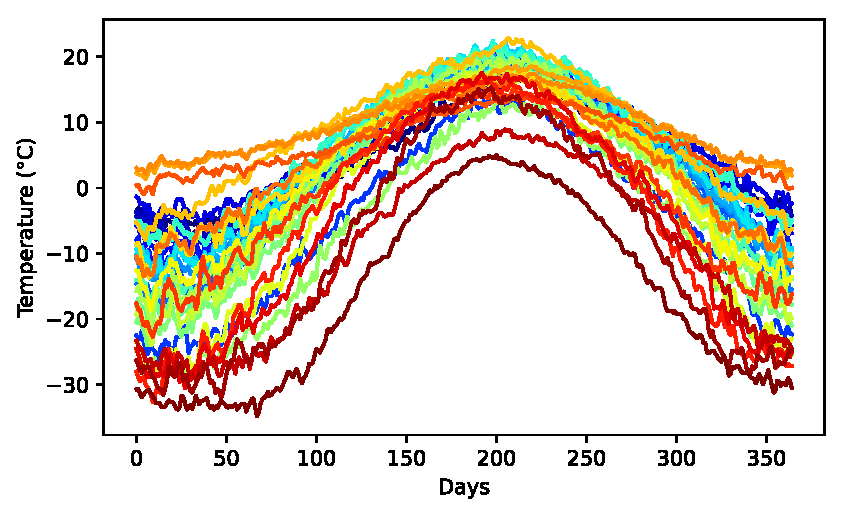
\includegraphics[width=0.49\textwidth]{temperature.eps}
    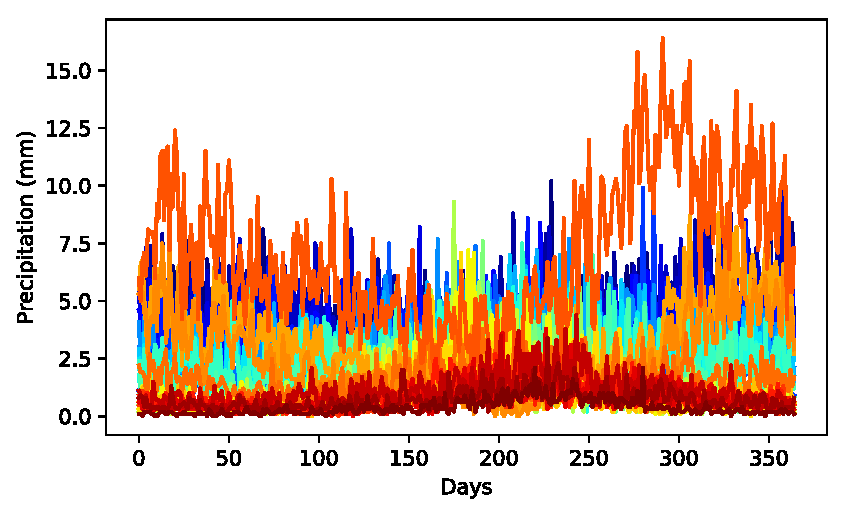
\includegraphics[width=0.49\textwidth]{precipitation.eps}
    \caption{Canadian weather dataset.}
    \label{fig:canadian_weather}
\end{figure}

\textcolor{blue}{We estimate the functional principal components using the \texttt{Gram}, \texttt{(Tensor) PCA} and \texttt{2D/1D B-Splines} methods from the Canadian weather dataset. Prior to applying each method, the data was smoothed using P-splines with a fixed penalty. For the \texttt{(Tensor) PCA} method, the estimation of the multivariate eigenfunctions is based on the univariate estimation of $5$ univariate eigenfunctions. For the \texttt{2D/1D B-splines} method, the two components are expanded in $13$ B-splines.  Figure~\ref{fig:canadian_weather_eigenfunctions} presents the results of MFPCA retaining the top three principal components. Recalling that eigenfunctions are defined up to a sign, the results across all three methods are similar. Our analysis focuses on the Gram method's results. The first principal component (red) exhibits positive values for both temperature and precipitation, indicating that weather stations with positive scores will experience above-average temperatures and precipitation. This effect is more pronounced during winter than summer, as the eigenfunctions approach zero during the summer months. Similar interpretations can be applied to the remaining eigenfunctions.}
\begin{figure}
    \centering
    \begin{subfigure}[b]{0.3\textwidth}
    \centering
    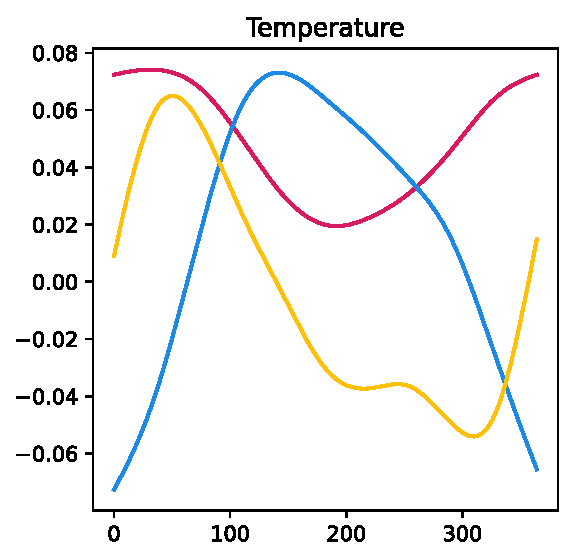
\includegraphics[width=\textwidth]{eigen_temp_gram.eps}
    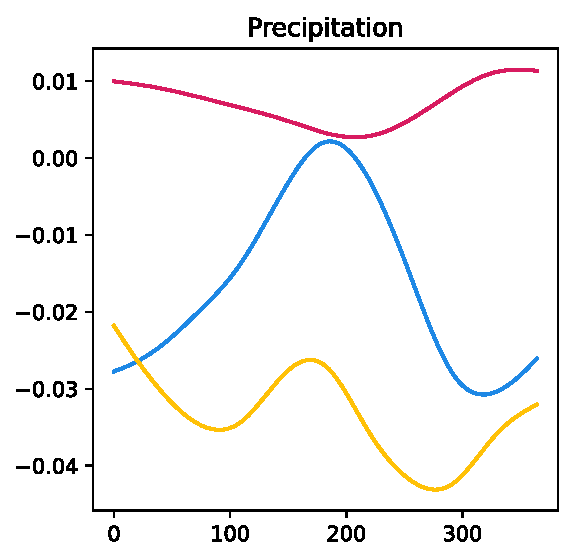
\includegraphics[width=\textwidth]{eigen_prec_gram.eps}
    \caption{\texttt{Gram} method.}
    \end{subfigure}
    \hfill
    \begin{subfigure}[b]{0.3\textwidth}
    \centering
    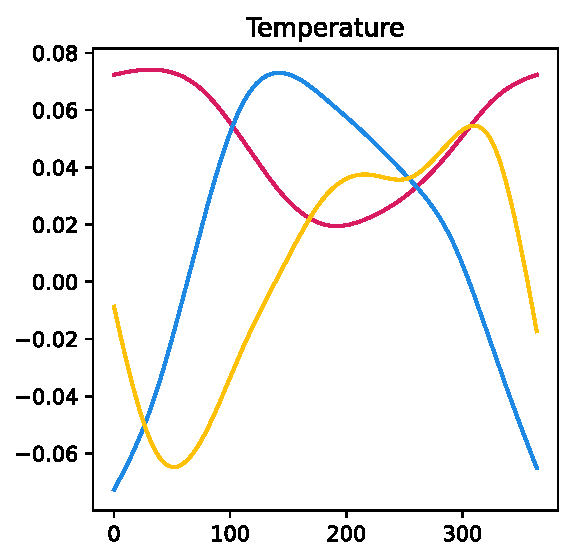
\includegraphics[width=\textwidth]{eigen_temp_cov.eps}
    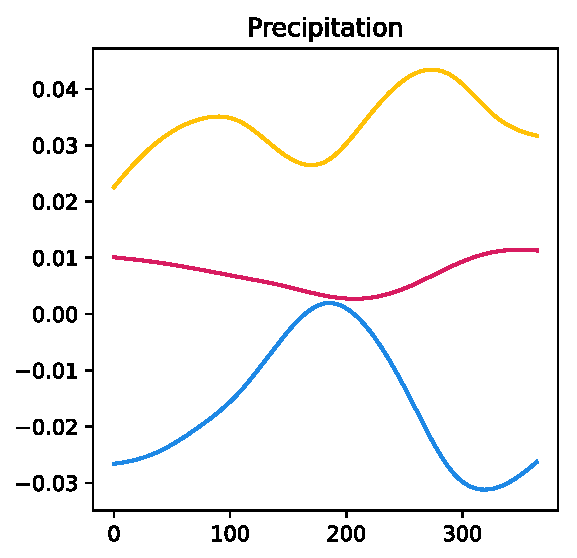
\includegraphics[width=\textwidth]{eigen_prec_cov.eps}
    \caption{\texttt{(Tensor) PCA} method.}
    \end{subfigure}
    \hfill
    \begin{subfigure}[b]{0.3\textwidth}
    \centering
    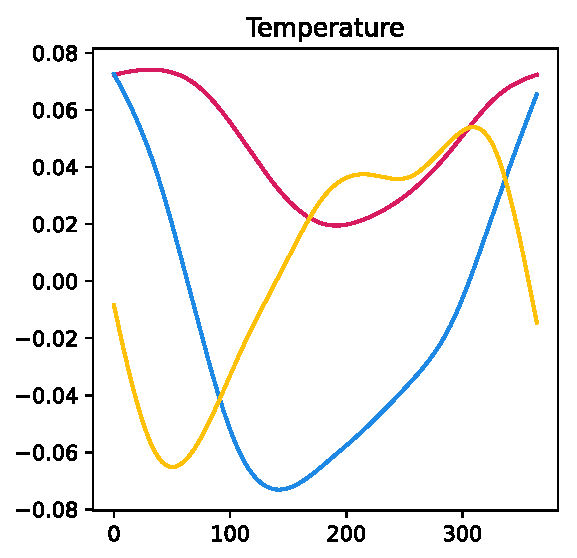
\includegraphics[width=\textwidth]{eigen_temp_psplines.eps}
    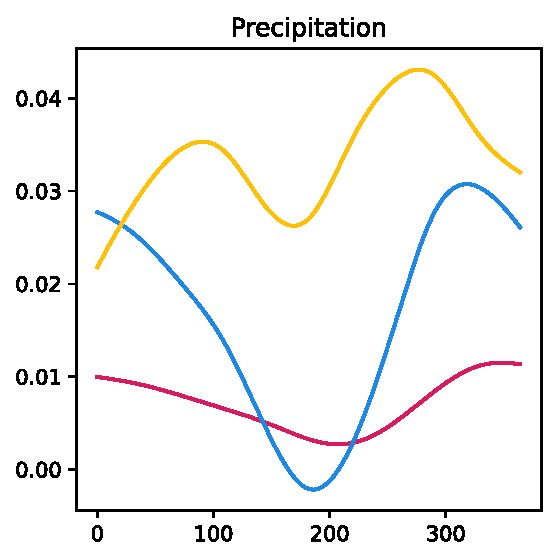
\includegraphics[width=\textwidth]{eigen_prec_psplines.eps}
    \caption{\texttt{2D/1D B-Splines} method.}
    \end{subfigure}
    \caption{The estimated eigenfunctions for the Canadian weather dataset using the different methods.}
    \label{fig:canadian_weather_eigenfunctions}
\end{figure}


% section canadian_weather (end)


% REFERENCES ---------
\bibliographystyle{apalike}
\bibliography{biblio}

\makeatletter\@input{ms_ref.tex}\makeatother
\end{document}

